\documentclass{article}
\usepackage{arxiv}

\usepackage[utf8]{inputenc} % allow utf-8 input
\usepackage[T1]{fontenc} % use 8-bit T1 fonts
\usepackage{hyperref} % hyperlinks
\usepackage{url} % simple URL typesetting
\usepackage{booktabs} % professional-quality tables
\usepackage{amsfonts} % blackboard math symbols
\usepackage{nicefrac} % compact symbols for 1/2, etc.
\usepackage{microtype} % microtypography
\usepackage{lipsum}
\usepackage{graphicx}
\usepackage{xcolor}
\usepackage{tabularx}
\usepackage{multicol}
\usepackage{amsmath}
\usepackage{caption}
\usepackage{array, multirow}

\usepackage{tikz}
\usetikzlibrary{shapes.geometric, arrows, positioning, fit}
\tikzstyle{startstop}
=
[rectangle,
rounded
corners,
minimum
width=3cm,
minimum
height=1cm,
text
centered,
draw=black,
fill=red!30]
\tikzstyle{process}
=
[rectangle,
minimum
width=3cm,
minimum
height=1cm,
text
centered,
draw=black,
fill=blue!30]
\tikzstyle{decision}
=
[diamond,
minimum
width=3cm,
minimum
height=1cm,
text
centered,
draw=black,
fill=green!30]

\tikzstyle{data}
=
[trapezium,
trapezium
left
angle=70,
trapezium
right
angle=110,
minimum
width=3cm,
minimum
height=1cm,
text
centered,
draw=black,
fill=green!30]
\tikzstyle{arrow}
=
[thick,->,>=stealth]
\tikzstyle{group}
=
[rectangle,
dashed,
draw=black,
inner
sep=0.25cm]
\tikzstyle{action}
=
[rectangle,
draw=black,
inner
sep=0.2cm,
text
centered,
font=\scriptsize]

\date{}

\captionsetup{skip=2pt}

\title{Machine Learning Application \\ Land Owner's Willingness to Sell \emph{} }
\author{ Amanda G Foess \\ Stanford University \\ Bachelor of Science in Computer
Science \\ CS 229: Machine Learning Theory \\ \texttt{agfoess@stanford.edu} \\ }

% Redefine maketitle to exclude the date
\makeatletter
\renewcommand{\maketitle}{
\begin{center}
	{\LARGE \@title \par} \vskip 1.5em
	{\large \lineskip .5em \begin{tabular}[t]{c}\@author\end{tabular}\par} \vskip
	1em
\end{center}
}
\makeatother

\begin{document}
	\maketitle
	\section{Introduction}

The finished home price to land value ratio is a fundamental metric in land development,
representing how much of a house's total value comes from the land itself. This ratio
plays a pivotal role in evaluating the financial viability of real estate projects,
particularly in mass production housing. By analyzing and tracking this ratio across
various submarkets, developers can make more precise financial decisions
regarding raw land acquisition and project planning, aligning development strategies
with market conditions.

\[
	\text{Ratio}= \frac{ \text{Market retail sale price of a new finished home} }{
	\text{Vacant developed lot price the builder pays the developer} }
\]

This ratio is determined by two main components: (1) the market value of the finished
property, influenced by factors such as location, size, and sales of comparable
properties, and (2) the price of a vacant developed lot (VDL) that builders are willing
to pay, which is calculated using the residual land valuation method. A well-balanced
ratio signals that development costs align with the land’s worth, suggesting a
potentially profitable project. On the other hand, a skewed ratio could mean the
project is burdened with high costs or that the land’s value is underestimated, prompting
the need for further financial evaluation. For developers, understanding this ratio
across the broader market, submarkets, and individual builder preferences allows
for accurate lot pricing, ensuring builders can achieve their desired internal
profit margins.

Estimating this ratio accurately is no small task, as it requires navigating a range
of challenges. Real estate markets are inherently dynamic, influenced by fluctuating
economic conditions, interest rates, and local developments. Market-specific
factors, such as neighborhood appeal, proximity to amenities, and future development
potential, also significantly impact the ratio but are difficult to quantify
precisely. In addition, zoning regulations, land-use policies, and environmental
rules introduce further complexity. Traditional valuation methods, while
valuable, often rely on detailed financial forecasts and assumptions that can introduce
uncertainty.

This study applies a machine learning approach, using XGBoost, to predict the finished
home price to land value ratio at the early stages of a project. This proactive
approach shifts the focus from traditional reactive calculations—performed after
significant project data has been finalized—to early-stage predictions that
empower stakeholders to make informed decisions right from the outset.

The model integrates diverse data sources, including numeric inputs such as acreage,
estimated Vacant Developed Lot (VDL) sale prices, and geospatial details (latitude,
longitude, and sale date), as well as categorical features like land usage and
grantee mappings. By leveraging these inputs, the model uncovers complex
patterns and relationships that influence the predicted finished lot price to
land value ratio.

This research contributes to the development of more efficient land valuation
practices, aiding in the supply of affordable housing and addressing housing shortages
in high-demand areas. By improving the accuracy of this critical ratio and
adapting it to localized submarket conditions, the study offers a powerful tool for
strategic decision-making in land development.

	\section{Related Work}

Gu et al. (2023) explored the application of machine learning models to predict
land development intensity, a critical metric for understanding the efficiency of
land use and guiding regional planning. Their study compared four
algorithms—XGBoost, Random Forest, Support Vector Machine, and Decision Tree—and
found that XGBoost outperformed the others, achieving an $R^{2}$ of 95.66\% and an
MSE of 0.16. This research underscores the utility of XGBoost in modeling
complex relationships between natural, social, and economic factors influencing
land development.\cite{gu2023landdevelopment}.

	\section{Dataset \& Features}

%  "download data"
\textbf{(1) Download Raw Data:} The raw data is downloaded from the Mecklenburg
County ArcGIS Sales platform, providing a .csv file containing property sales
data. The dataset includes various features, as outlined in Table 1.
\begin{table}[h!]
	\centering
	\caption{Features in the Raw Data}
	\renewcommand{\arraystretch}{1} % Reduce row height
	\setlength{\tabcolsep}{8pt} % Reduce column padding
	\begin{tabular}{|l|l|l|l|l|l|l|l|}
		\hline
		\texttt{parcelid}   & \texttt{transferid} & \texttt{propertyid} & \texttt{saleprice} & \texttt{saledate} & \texttt{soldasvaca} & \texttt{landuseful}  & \texttt{landuse}     \\
		\hline
		\texttt{deeddescri} & \texttt{legalrefer} & \texttt{salesvalid} & \texttt{naldesc}   & \texttt{grantor}  & \texttt{grantee}    & \texttt{shape\_Leng} & \texttt{shape\_Area} \\
		\hline
	\end{tabular}
\end{table}

% "(2) WebScraping/processArcGISSales.py"
\textbf{(2) Data Cleaning:} A Python script processes the raw data in chunks of
10,000 rows for efficient handling of large data volumes. The cleaning process involves:
(1) dropping rows with missing \texttt{transferid} or \texttt{parcelid}, (2) removing
records with \texttt{saleprice} equal to 0, and (3) discarding columns that are not
required for subsequent analysis.

\textbf{(3) Feature Engineer [Acres]:} The feature \texttt{Acres} is calculated by
converting the raw \texttt{shape\_Area} values from square feet to acres.

\textbf{(4) Feature Engineer [VDL Sale Price]:} The feature \texttt{VDL Sale
Price} is computed by dividing \texttt{saleprice} by the count of records sharing
the same \texttt{transferid}. This adjustment accounts for multiple parcels associated
with a single transaction.

% "(3) TransformData/2_findHomeToLotRatio.py"
\textbf{(5) Feature Engineer [Adjusted Finished Home Value]:} For records with
unique \texttt{Home Transfer ID}, the corresponding Finished Home Value is
divided by the count of properties linked to that ID. This adjustment normalizes
the finished home value for cases involving multiple properties under a single transfer.

\textbf{(6) Feature Engineer [House to Lot Ratio]:} The \texttt{House to Lot
Ratio} is determined by dividing the \texttt{Adjusted Finished Home Value} by
the \texttt{VDL Sale Price}, provided the latter is non-zero.

% "(3) TransformData/3_queryRecordAddress.py"
\textbf{(7) Feature Engineer [Latitude, Longitude]:} The script queries a public
GIS API to retrieve the first address associated with each \texttt{parcelid}. The
Google Geocoding API is then used to derive the geographical coordinates (latitude
and longitude) for parcels with valid addresses.

\begin{minipage}[t]{0.48\textwidth}
	\centering
	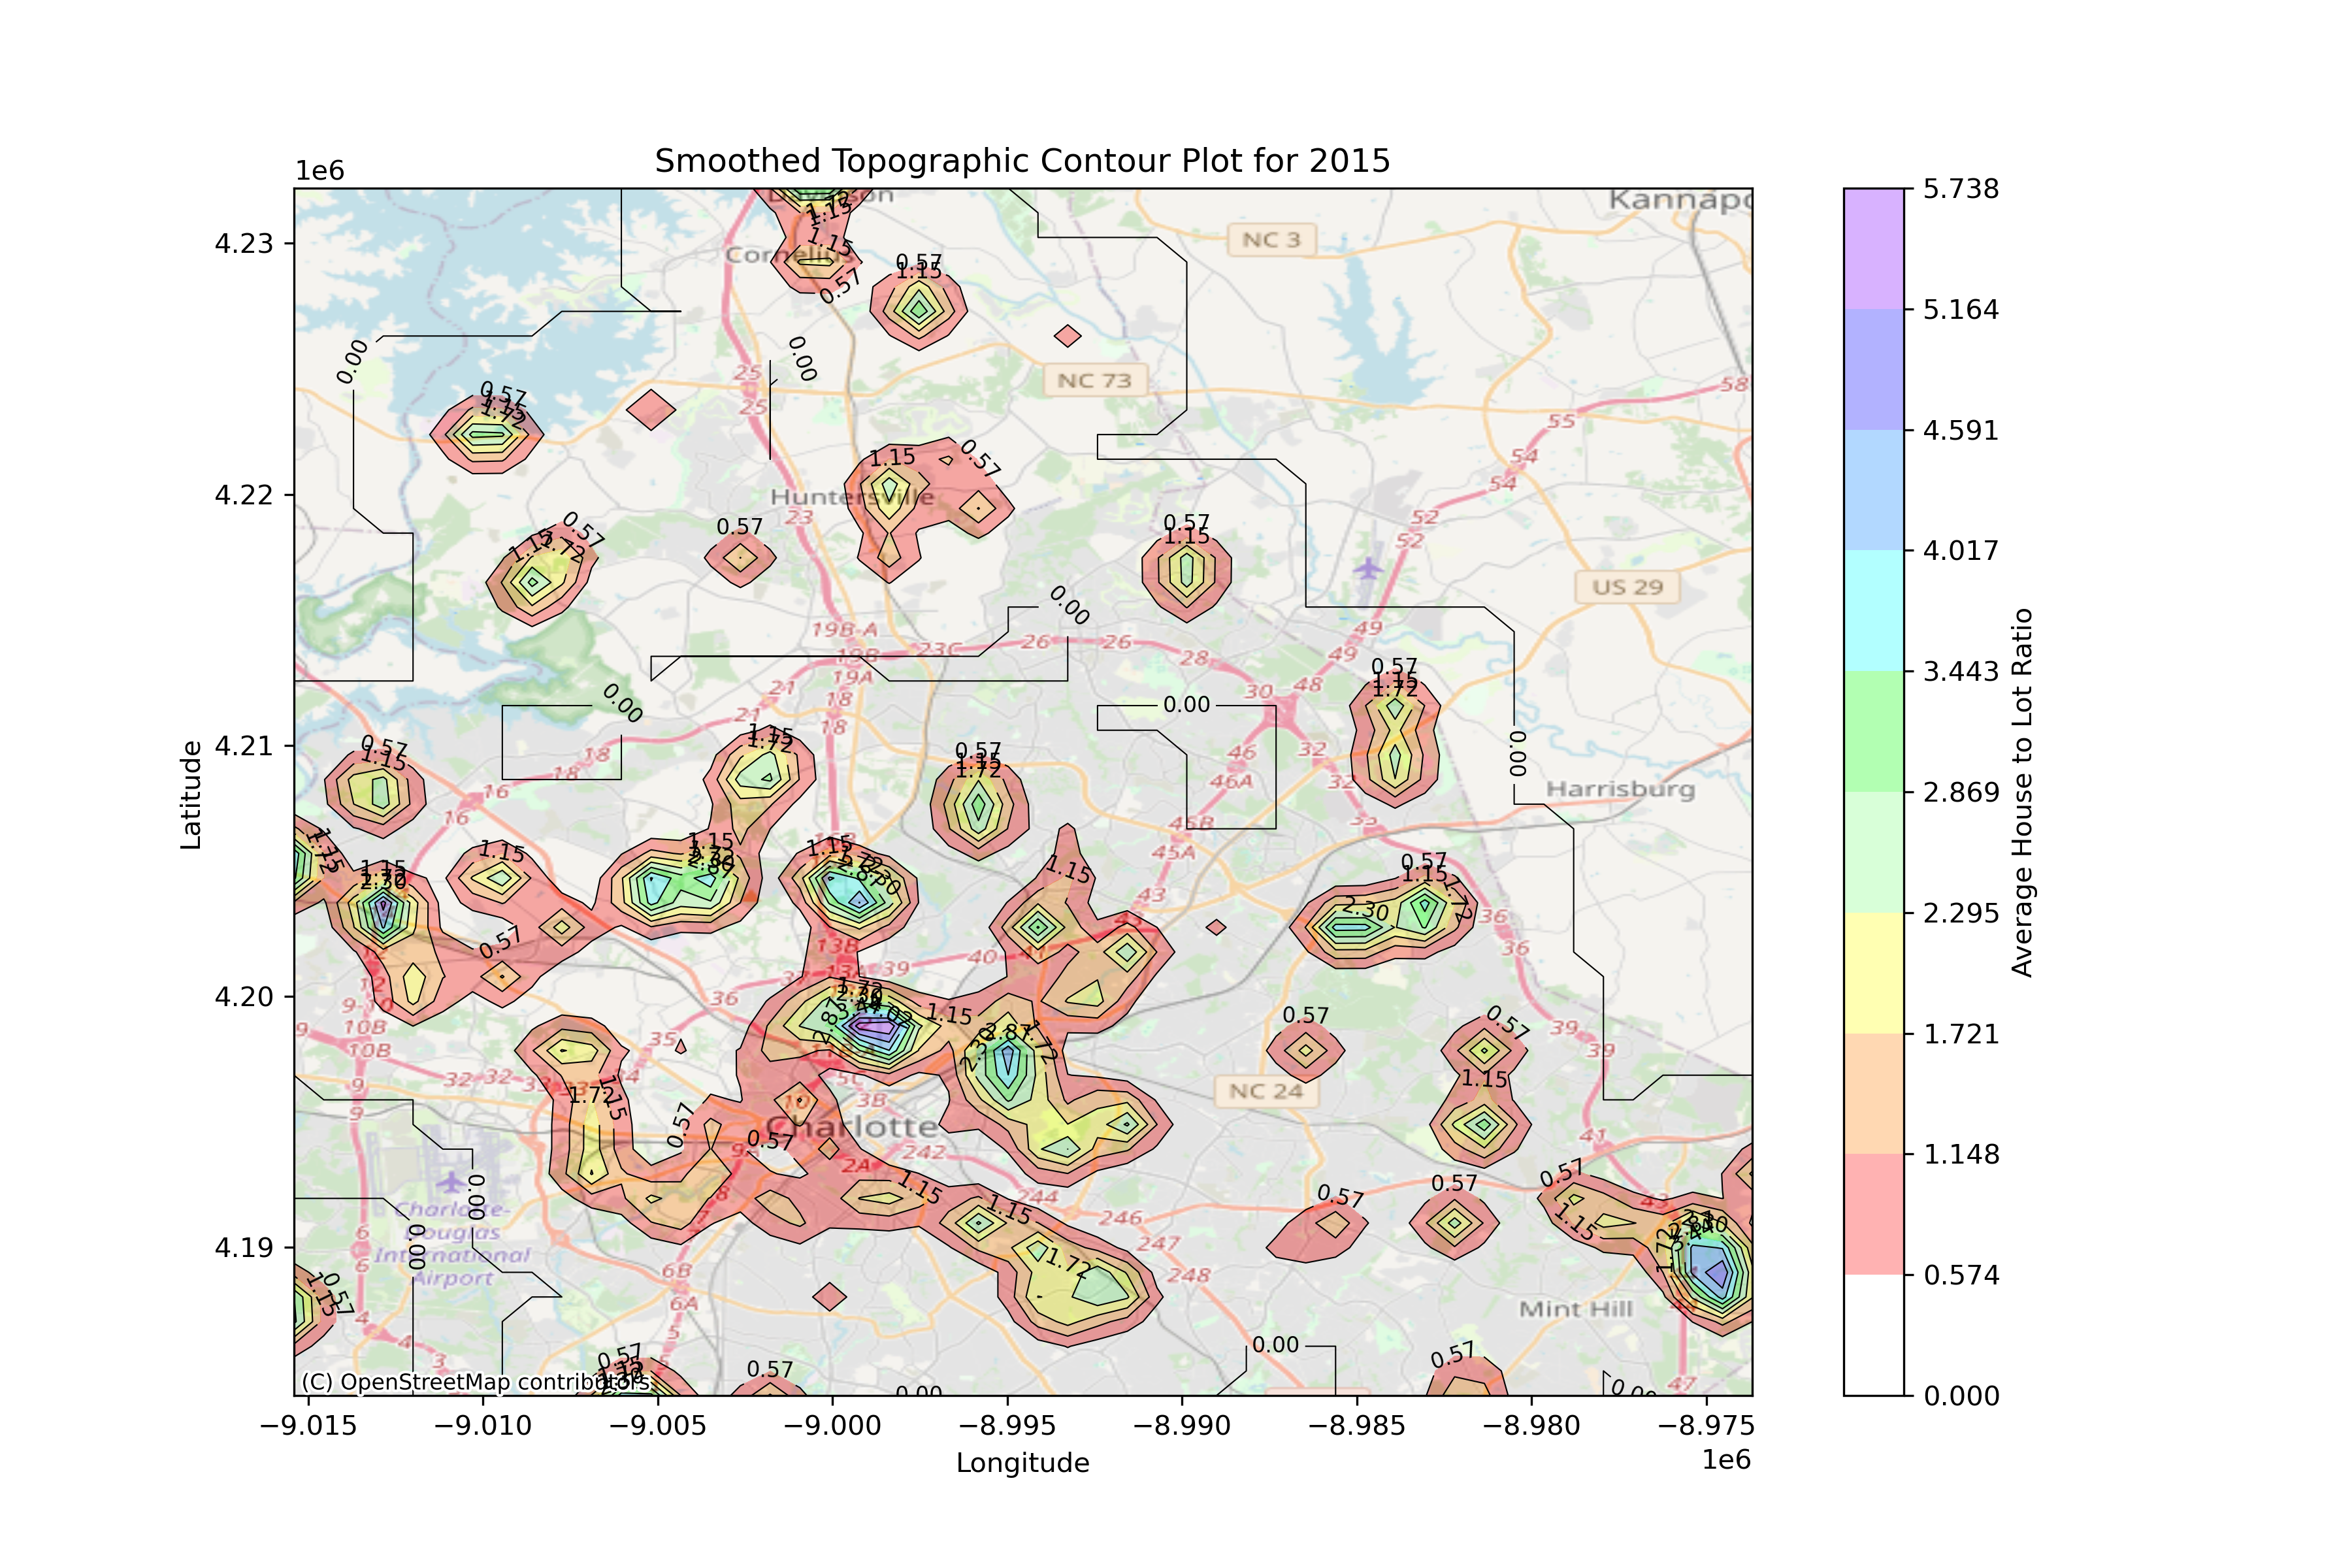
\includegraphics[width=\textwidth]{Sections/House_to_Lot_Ratio_2015.png}
	\captionof{figure}{Visual Mapping of House to Lot Ratio (2015)}
\end{minipage}%
\hfill
\begin{minipage}[t]{0.48\textwidth}
	\centering
	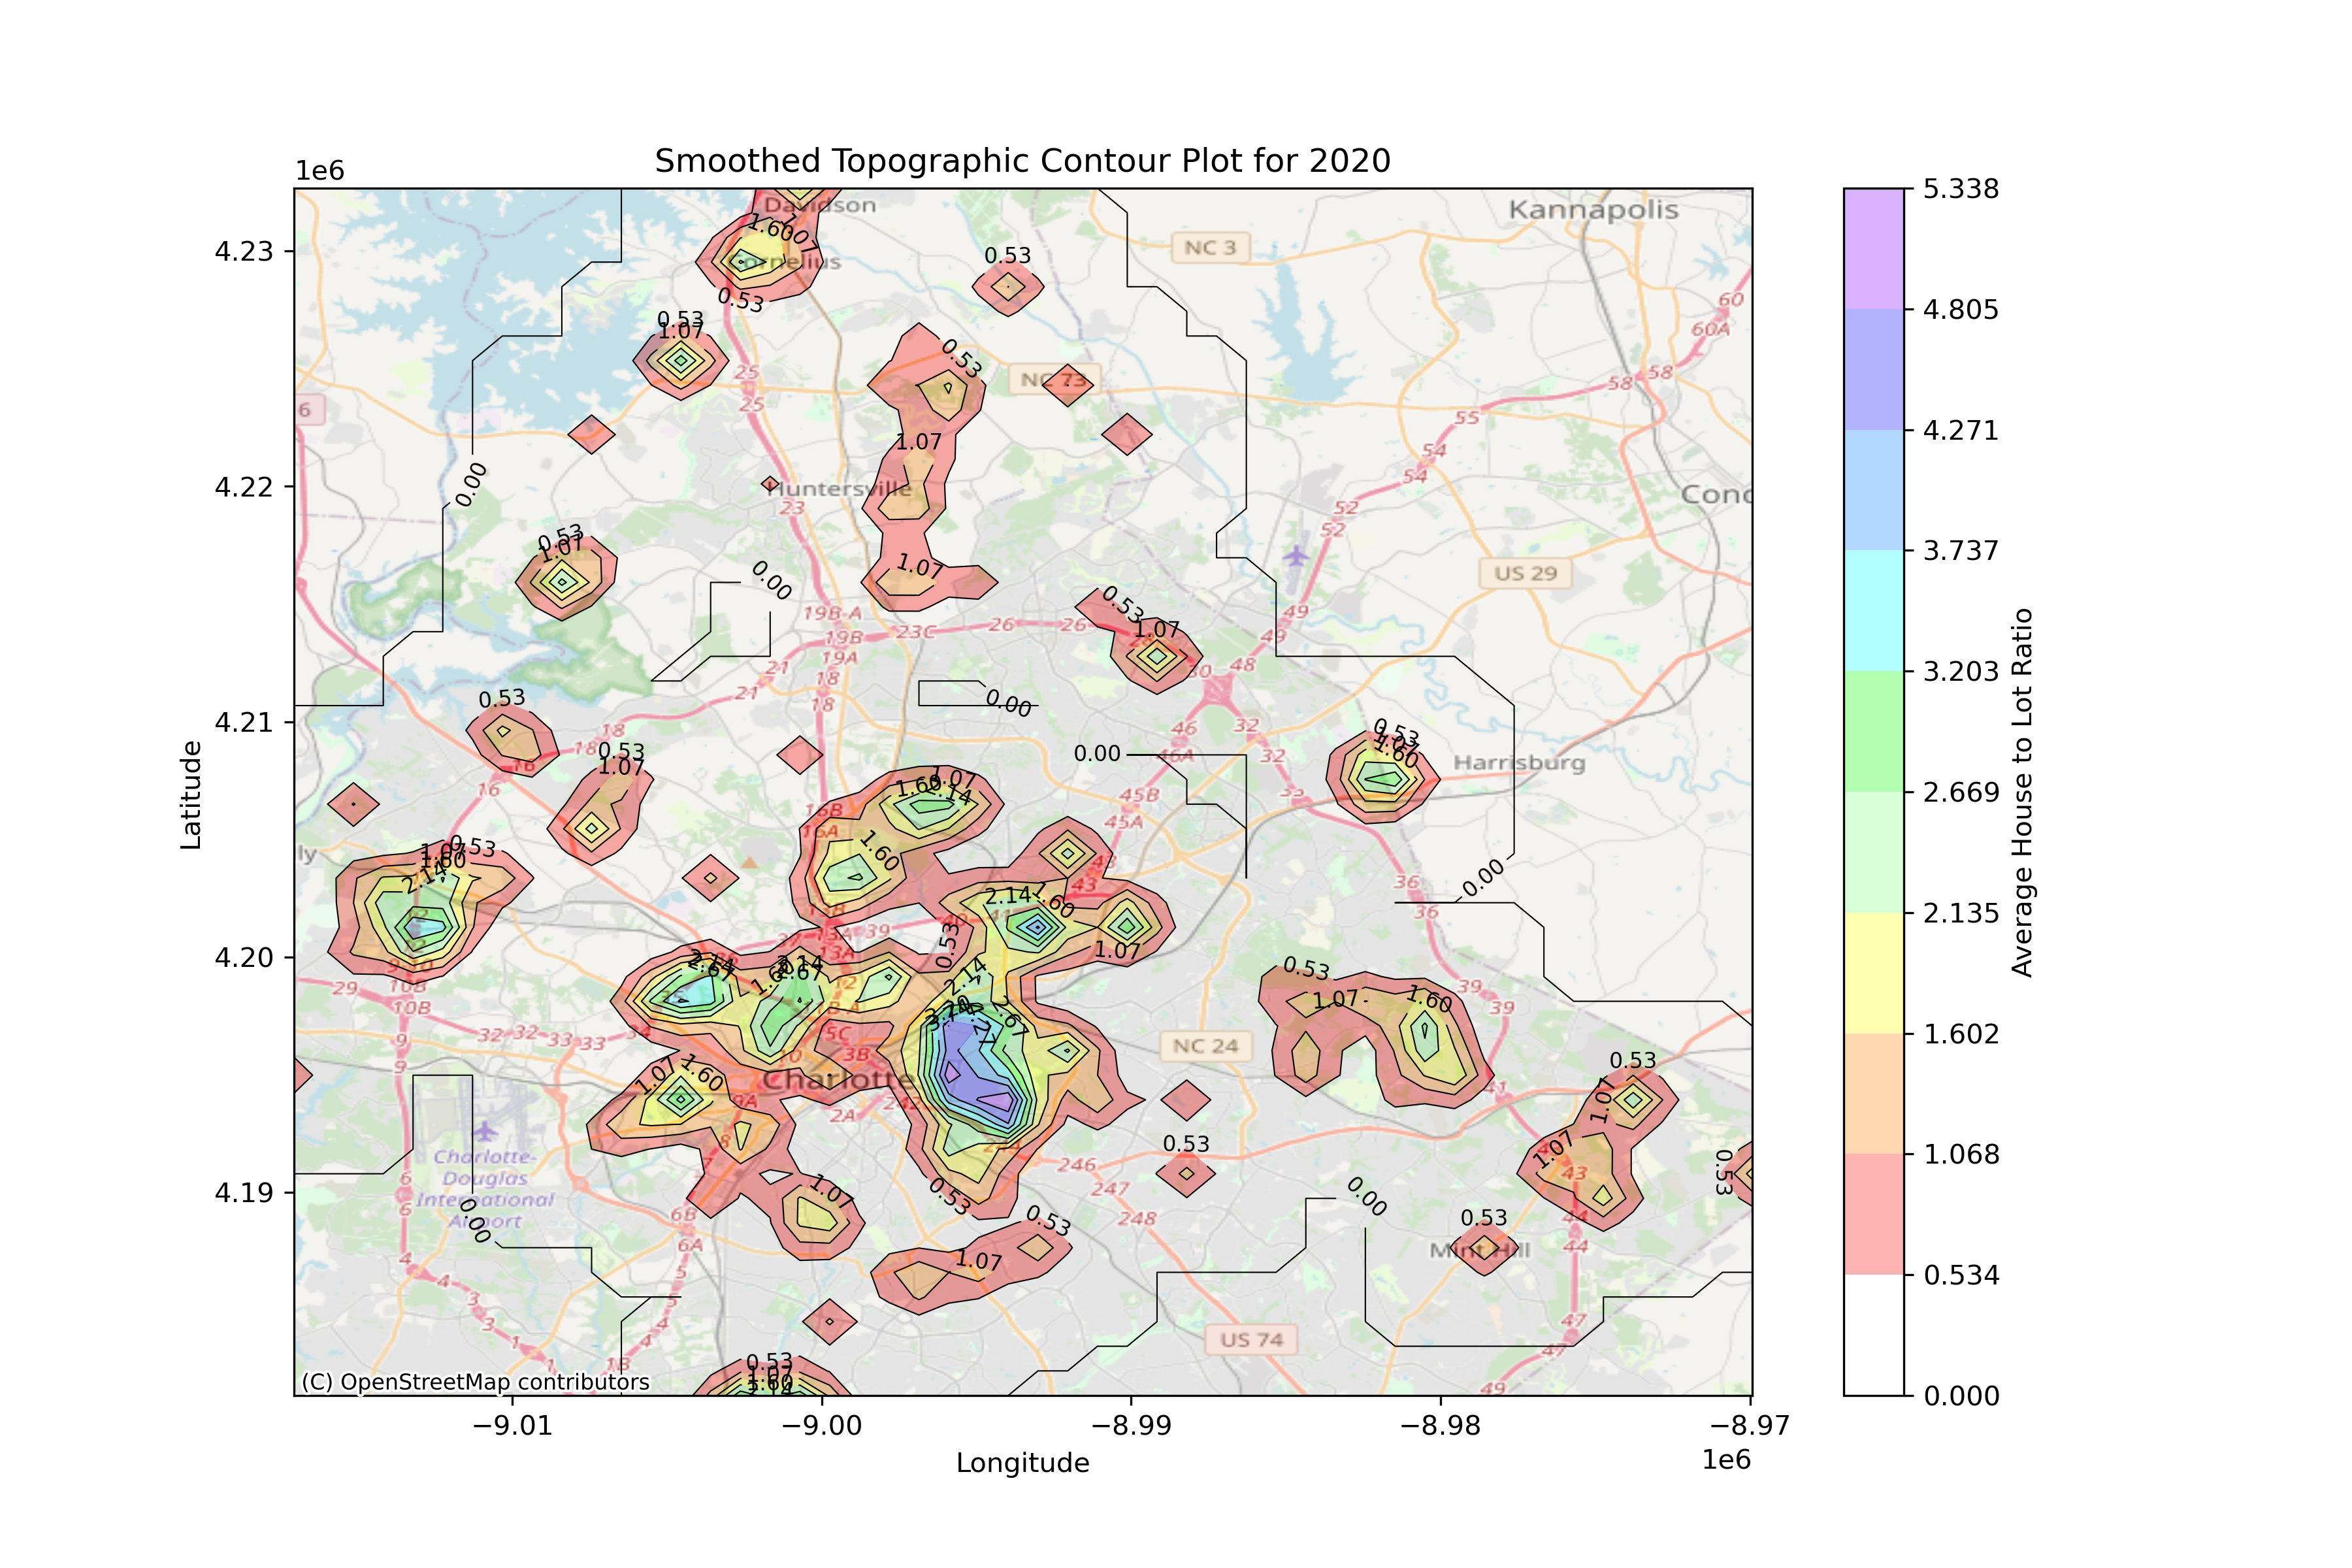
\includegraphics[width=\textwidth]{Sections/House_to_Lot_Ratio_2020.png}
	\captionof{figure}{Visual Mapping of House to Lot Ratio (2020)}
\end{minipage}

% "(3) TransformData/4_addFeatures.py"
\textbf{(8) Feature Modification [Landuse]:} Records are filtered based on a
predefined dictionary of land-use categories, which identifies land-use types to
"keep" or "drop." Only rows with land-use types marked as "keep" are retained. Examples
of "keep" categories are listed in Table 2.
\begin{table}[h!]
	\centering
	\caption{Land Use Features Marked as "Keep"}
	\renewcommand{\arraystretch}{1} % Reduce row height
	\setlength{\tabcolsep}{8pt} % Adjust column padding
	\begin{tabular}{|l|l|}
		\hline
		USE VALUE HOMESITE                  & SINGLE FAMILY RESIDENTIAL              \\
		\hline
		RURAL HOMESITE                      & SINGLE FAMILY RESIDENTIAL - COMMON     \\
		\hline
		SINGLE FAMILY RESIDENTIAL - ACREAGE & MULTI FAMILY GARDEN                    \\
		\hline
		TOWN HOUSE SFR                      & SINGLE FAMILY RESIDENTIAL - WATERFRONT \\
		\hline
		MULTI FAMILY                        & MULTI FAMILY DUPLEX/TRIPLEX            \\
		\hline
		SINGLE FAMILY RESIDENTIAL - GOLF    & MULTI FAMILY MARINA LAND               \\
		\hline
		SCHOOL, COLLEGE, PRIVATE            & SINGLE FAMILY RESIDENTIAL - RIVER      \\
		\hline
	\end{tabular}
\end{table}

% "(3) TransformData/4.23_addStandardizedGranteeNames.py"
\textbf{(9) Feature Engineer [Mapped Grantee]:} The \texttt{Mapped\_Grantee}
column is created by standardizing the \texttt{grantee} names using a dictionary-based
mapping. This eliminates variations in grantee names caused by inconsistent
formats or spellings. Records with grantee values appearing only once are excluded,
focusing on more frequent entities.
\begin{table}[h!]
	\centering
	\caption{Mapping Original Grantee Variations to Standardized Grantee (Example)}
	\renewcommand{\arraystretch}{1} % Adjust row height
	\setlength{\tabcolsep}{8pt} % Adjust column padding
	\begin{tabular}{|l|l|}
		\hline
		\textbf{Standardized Mapped Grantee}   & \textbf{Original Grantee Variations} \\
		\hline
		\multirow{4}{*}{D R HORTON-REGENT LLC} & D R HORTON INC                       \\
		                                       & D R HORTON REGENT LLC                \\
		                                       & D R HORTON                           \\
		                                       & D R HORTON INC                       \\
		\hline
	\end{tabular}
\end{table}

% "(3) TransformData/4.24_transformData.py"
\textbf{(10) Feature Modification [Saledate]:} The \texttt{saledate} column is
reformatted into a \texttt{YYYY-MM} format for consistency and ease of time-series
analysis.

% "(3) TransformData/4.25_findBestIQRGrid.py" "(3) TransformedData/4.26_transformData_BestIQRHypTuning.py"
\textbf{(11) Systematically Remove Outliers Using Inner Quartile Range:} The
script systematically removes outliers by applying IQR thresholds to features
such as \texttt{House to Lot Ratio}, \texttt{Acres}, and \texttt{VDL Sale Price}.
Threshold ranges between [0, 0.2] are tested iteratively, and the dataset is
filtered based on the optimal threshold values that maximize model performance. Outliers
are removed through the following steps: (1) calculate IQR for each feature, (2)
determine the lower and upper bounds using the threshold configuration, (3)
exclude records outside these bounds.
\[
	\begin{aligned}
		Q_{1}      & = \begin{cases}x_{k}&\text{if }n \cdot p \text{ is an integer, where }p = \text{bottom\_range}, \\ x_{\lfloor n \cdot p \rfloor + 1}&\text{otherwise},\end{cases}  \\
		Q_{3}      & = \begin{cases}x_{k}&\text{if }n \cdot p \text{ is an integer, where }p = 1 - \text{top\_range}, \\ x_{\lfloor n \cdot p \rfloor + 1}&\text{otherwise},\end{cases} \\
		\text{IQR} & = Q_{3}- Q_{1}, \quad \text{Lower Bound}= Q_{1}- 1.5 \cdot \text{IQR}, \quad \text{Upper Bound}= Q_{3}+ 1.5 \cdot \text{IQR}.
	\end{aligned}
\]
The model performance is evaluated on each configuration using $R^{2}$ and Mean Squared
Error (MSE). The best-performing thresholds are applied to the final dataset. A summary
of feature ranges and model test results is provided in Table 3 and Table 4,
respectively.
\begin{minipage}[t]{0.48\textwidth}
	\centering
	\captionof{table}{Feature Ranges}
	\renewcommand{\arraystretch}{1} % Adjust row height
	\begin{tabular}{|c|c|c|}
		\hline
		\textbf{Feature Name} & \textbf{Bottom} & \textbf{Top} \\
		\hline
		House to Lot Ratio    & 0.2             & 0.05         \\
		\hline
		Acres                 & 0.15            & 0.2          \\
		\hline
		VDL Sale Price        & 0.15            & 0.2          \\
		\hline
	\end{tabular}
\end{minipage}%
\hfill
\begin{minipage}[t]{0.48\textwidth}
	\centering
	\captionof{table}{Model Test Results}
	\renewcommand{\arraystretch}{1} % Adjust row height
	\begin{tabular}{|c|c|}
		\hline
		\textbf{Metric} & \textbf{Value} \\
		\hline
		Records Used    & 14735          \\
		\hline
		$R^{2}$ Test    & 0.903          \\
		\hline
		MSE Test        & 19.850         \\
		\hline
	\end{tabular}
\end{minipage}

The following section presents statistical summaries and distribution graphs for
the dataset, providing a visual and numerical overview of key features. These insights
help to highlight patterns, trends, and potential anomalies, forming the
foundation for subsequent analysis and model development.

\begin{minipage}[t]{0.3\textwidth}
	\centering
	\includegraphics[width=\linewidth]{
		Sections/ratio_distribution.png
	} % Replace with your image file
	\captionof{figure}{Feature Distribution: [Ratio]} % Caption for the second image
\end{minipage}%
\hfill
\begin{minipage}[t]{0.3\textwidth}
	\centering
	\includegraphics[width=\linewidth]{
		Sections/acre_distribution.png
	} % Replace with your image file
	\captionof{figure}{Feature Distribution: [Acre]} % Caption for the third image
\end{minipage}

The distributions of the data are not weighted uniformly, indicating potential imbalances
or biases in the dataset. This uneven distribution will need to be carefully
addressed during model development to ensure accurate and reliable predictions.

% "(3) TransformedData/4.26_transformData_BestIQRHypTuning.py"

	\section{Methods}

In our analysis, we employed three distinct regression techniques: Linear Regression,
Random Forest Regression, and XGBoost Regression. Each method offers unique
advantages and operates under different principles, allowing us to evaluate their
performance across various datasets.

Linear Regression serves as the baseline approach in regression analysis. It
models the relationship between a dependent variable and one or more independent
variables by fitting a linear equation to observed data. This simplicity facilitates
straightforward interpretation of coefficients, making it ideal for datasets
where relationships are expected to be linear. However, its performance can
decline when dealing with complex, non-linear interactions among variables.

To address non-linear relationships, we utilized Random Forest Regression, an ensemble
learning method that constructs multiple decision trees during training. By
averaging the predictions from these individual trees, Random Forests enhance predictive
accuracy and control overfitting. This method captures intricate data patterns
and interactions, providing robust performance across diverse datasets. Notably,
Random Forests are less sensitive to noisy data and typically offer stable performance
across various scenarios.
\[
	\hat{y}= \frac{1}{N_{t}}\sum_{i=1}^{N_t}h_{i}(x)
\]
Further enhancing our modeling capabilities, we applied XGBoost Regression (Extreme
Gradient Boosting), an advanced ensemble technique that builds decision trees
sequentially. Each new tree focuses on correcting errors made by its predecessors,
optimizing performance through gradient descent algorithms. XGBoost is renowned for
its speed and efficiency, often delivering superior predictive accuracy, especially
in datasets with complex structures. However, it can be more sensitive to noisy data
and may overfit if not properly regularized.

The prediction model is:
\[
	\hat{y}_{i}= \sum_{k=1}^{K}f_{k}(x_{i}), \quad f_{k}\in \mathcal{F}
\]
where $f_{k}(x_{i})$ is the prediction from the $k$-th tree, and $\mathcal{F}$ is
the space of trees defined as:
\[
	\mathcal{F}= \{f(x) = w_{q(x)}\}, \quad q(x) \to T, \quad w \in \mathbb{R}^{T}
\]
The objective function is:
\[
	\mathcal{L}= \sum_{i=1}^{n}l(y_{i}, \hat{y}_{i}) + \sum_{k=1}^{K}\Omega(f_{k}),
	\quad \Omega(f) = \gamma T + \frac{1}{2}\lambda \|w\|^{2}
\]
where $l(y_{i}, \hat{y}_{i})$ is the loss function, $\gamma$ penalizes the
number of leaves $T$, and $\lambda$ regularizes the leaf weights.

To optimize the performance of our XGBoost regression model, we implemented a
hyperparameter tuning process using grid search. This method evaluates combinations
of hyperparameters to identify the configuration that maximizes the model's predictive
accuracy.

\begin{table}[h!]
	\centering
	\caption{Tuning Parameters and Their Tested Values}
	\renewcommand{\arraystretch}{1} % Adjust row height for better readability
	\setlength{\tabcolsep}{10pt} % Adjust column spacing
	\begin{tabular}{|l|l|}
		\hline
		\textbf{Parameter Name}    & \textbf{Tested Values}       \\
		\hline
		\texttt{n\_estimators}     & 300, 500, 700                \\
		\hline
		\texttt{max\_depth}        & 6, 8, 10                     \\
		\hline
		\texttt{learning\_rate}    & 0.1                          \\
		\hline
		\texttt{subsample}         & 1.0                          \\
		\hline
		\texttt{colsample\_bytree} & 0.4, 0.6, 0.8                \\
		\hline
		\texttt{reg\_alpha}        & 0, 0.05, 0.1, 0.15, 0.2, 0.5 \\
		\hline
		\texttt{reg\_lambda}       & 0, 0.2, 0.4, 0.6, 0.8, 1.0   \\
		\hline
	\end{tabular}
\end{table}
First, we explored tree structure by varying the number of boosting rounds (n\_estimators)
and the depth of the trees (max\_depth). These parameters helped us balance the trade-off
between underfitting (where the model is too simple to capture patterns) and overfitting
(where the model is overly complex and sensitive to noise). To further manage
overfitting, we incorporated regularization through parameters like reg\_alpha (L1
regularization) and reg\_lambda (L2 regularization), which penalize large
weights or excessive complexity.

Feature sampling was another focus, where we adjusted colsample\_bytree to test how
using fewer features per tree impacted the model's stability and robustness.
Additionally, the learning rate controlled the step size during optimization,
and subsampling was used to evaluate how reducing the number of samples affected
the model’s generalization.

To streamline the tuning process, we implemented Scikit-learn's GridSearchCV for
hyperparameter optimization. The XGBoost model was incorporated into a pipeline,
ensuring consistent preprocessing and hyperparameter testing. We applied three-fold,
five-fold, and ten-fold cross-validation to assess the model's performance
across different data splits, using the $R^{2}$ score as our evaluation metric.
This score measures the proportion of variance explained by the model, providing
a clear benchmark for predictive accuracy.

By employing these three regression methods, we aimed to capture a broad
spectrum of data relationships, from simple linear trends to complex, non-linear
interactions.

	\section{Experiments / Results / Discussion}

\textbf{Random Forest Model:} The results from the Random Forest model, with a training
MSE of 1.92 and test MSE of 2.37, and $R^{2}$ scores of 0.77 for training and
0.72 for testing, indicate moderate predictive performance.

\begin{table}[h!]
	\centering
	\caption{Random Forest Model Performance Metrics}
	\renewcommand{\arraystretch}{1} % Adjust row height for better readability
	\setlength{\tabcolsep}{10pt} % Adjust column spacing
	\begin{tabular}{|c|c|c|}
		\hline
		\textbf{Metric} & \textbf{Training} & \textbf{Test} \\
		\hline
		MSE             & 1.92              & 2.37          \\
		\hline
		$R^{2}$         & 0.77              & 0.72          \\
		\hline
	\end{tabular}
\end{table}

The small gap between the training and test metrics shows that the Random Forest
model avoids overfitting, which is a positive outcome. However, the $R^{2}$ value
of 0.72 for the test set indicates that nearly 28\% of the variance remains
unexplained, suggesting there is room for improvement in predictive accuracy.
Additionally, Random Forest, while robust, treats each tree independently and averages
their results, which can sometimes limit its ability to capture complex
relationships or interactions in high-dimensional data.

The Random Forest model serves as a strong baseline, demonstrating good generalization
and predictive capacity. However, the unexplained variance and potential limitations
in capturing complex feature interactions make XGBoost a compelling next step.
With its advanced boosting mechanism, regularization capabilities, and efficient
handling of high-dimensional data, XGBoost offers the potential to achieve higher
accuracy and better $R^{2}$ scores, ultimately leading to more reliable
predictions for the finished lot price to land value ratio.

\textbf{Final Model Training Details:} The final machine learning regression model
underwent an extensive hyperparameter tuning process, involving 5-fold cross-validation
over 972 hyperparameter combinations, resulting in a total of 4860 fits. This
thorough optimization ensures that the model achieves both robust performance
and generalizability.

\begin{minipage}[t]{0.48\textwidth}
	\centering
	\captionof{table}{Best Hyperparameters for the Model}
	\renewcommand{\arraystretch}{1} % Adjust row height
	\setlength{\tabcolsep}{8pt} % Adjust column spacing
	\begin{tabular}{|l|c|}
		\hline
		\textbf{Parameter Name}                 & \textbf{Value} \\
		\hline
		\texttt{regressor\_\_colsample\_bytree} & 0.4            \\
		\hline
		\texttt{regressor\_\_learning\_rate}    & 0.1            \\
		\hline
		\texttt{regressor\_\_max\_depth}        & 10             \\
		\hline
		\texttt{regressor\_\_n\_estimators}     & 700            \\
		\hline
		\texttt{regressor\_\_reg\_alpha}        & 0.5            \\
		\hline
		\texttt{regressor\_\_reg\_lambda}       & 0              \\
		\hline
		\texttt{regressor\_\_subsample}         & 1.0            \\
		\hline
	\end{tabular}
\end{minipage}%
\hfill
\begin{minipage}[t]{0.48\textwidth}
	\centering
	\captionof{table}{Model Performance Metrics}
	\renewcommand{\arraystretch}{1} % Adjust row height
	\setlength{\tabcolsep}{10pt} % Adjust column spacing
	\begin{tabular}{|c|c|c|}
		\hline
		\textbf{Metric} & \textbf{Training} & \textbf{Test} \\
		\hline
		MSE             & 2.06              & 3.66          \\
		\hline
		$R^{2}$         & 0.91              & 0.85          \\
		\hline
	\end{tabular}
\end{minipage}

The optimized hyperparameters include a maximum depth of 10 for the decision
trees, allowing the model to capture complex patterns without overfitting. The
learning rate was set to 0.1, providing a balanced trade-off between convergence
speed and model stability. Regularization parameters (\texttt{reg\_alpha} and
\texttt{reg\_lambda}) were adjusted to reduce overfitting, with \texttt{reg\_alpha}
set to 0.5 and \texttt{reg\_lambda} set to 0. The model also used a subsample value
of 1.0 and a \texttt{colsample\_bytree} value of 0.4, ensuring sufficient diversity
in the trees while controlling complexity.

The slight drop in performance from the training to the test set suggests the model
generalizes well, but it also indicates there may still be minor overfitting or
limitations in capturing the full variability of unseen data.

\begin{figure}[h!]
	\centering
	\includegraphics[width=0.3\textwidth]{
		Sections/Final Model.png
	} % Replace with your image path
	\caption{Predicted vs Actual House-to-Lot Ratio}
\end{figure}

	\section{Conclusion and Future Works}

The development and implementation of an XGBoost regression model for predicting
the finished lot price to land value ratio have demonstrated significant potential
in aiding land development decision-making. Rigorous hyperparameter tuning
ensured robust performance, with the model achieving an $R^{2}$ score of 0.91 on
the training set and 0.85 on the test set, along with a low Mean Squared Error (MSE).
These metrics indicate strong predictive capability and minimal overfitting,
making the model a reliable tool for early-stage project assessments.

While the model performs well, there are several avenues for future research and
development. Exploring advanced geospatial techniques or incorporating proximity-based
metrics (e.g., distance to amenities, transport hubs) could provide a deeper understanding
of location-specific influences. Developing a temporal model that accounts for
time-series data could help track and predict trends in the ratio over time, improving
its utility for long-term planning.

	\section{Contributions}

This project was conducted by Amanda Foess, leveraging insights and guidance
from expert sources in the land development industry. Their expertise ensured the
study aligns with real-world practices and industry standards.

	\section{References}

\bibliography{../references.bib}

\url{https://github.com/AmandaFoess/CS229-Project}

@article{gu2023landdevelopment, author = {Gu, G. and Wu, B. and Zhang, W. and Lu, R. and Feng, X. and Others}, title = {Comparing Machine Learning Methods for Predicting Land Development Intensity}, journal = {PLOS ONE}, volume = {18}, number = {4}, pages = {e0282476}, year = {2023}, doi = {10.1371/journal.pone.0282476}, url = {https://doi.org/10.1371/journal.pone.0282476} }
\end{document}